\section{Deformable Model without Landmarks}

\begin{figure}[h!]
    \centering
        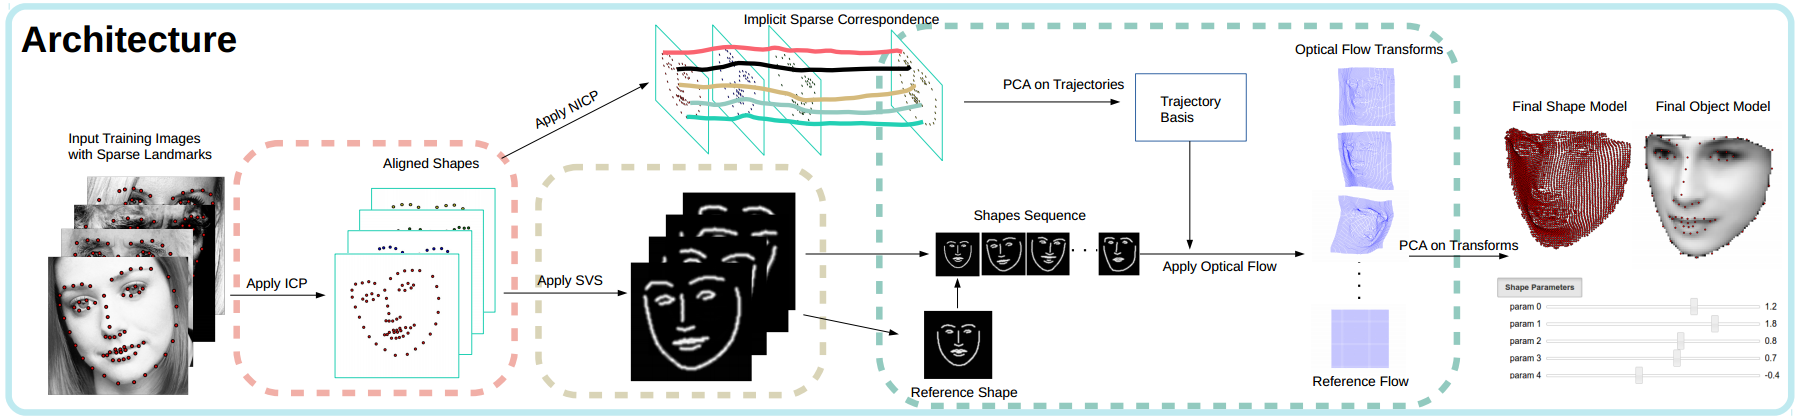
\includegraphics[width=0.5\textwidth]{resources/architecture}
    \caption{Training Architecture}
    \label{fig:archi}
\end{figure}

Deformable models is wildly used for object detection, localization, recognition and tracking while training a deformable model with good generalisation requires tremendous amount of carefully annotated data, which is extremely time consuming. Even more, annotated data normally requires same numbers of landmarks for one object category in every training data that exacerbated the cost of manual annotation. 

In addition, in contrast with sparse landmarks, dense shape reveals more nuanced structure. However, there is, to the best of our knowledge, no available densely annotated data set.

Our research proposed an architecture of accepting various annotations and structuring deformable model without using landmarks. Moreover, we proposed a new method of annotating data which is drawing. The architecture contains two major modules. The first modules handles inconsistent annotation set by converting to landmark independent shape discriminator. While the other module produces shape flow on object discriminators to generate dense flow transformations in shape space following by robust PCA\cite{?} to generate deformable model. In this section, we present the entire architectures, design decision and algorithms.

\subsection{Sparse Landmarks Pre-Processing}
The first module is to bridge the gap that training data has to have consistent number of landmarks. Currently existing annotated databases contains large variety on landmarking, which largely restricted model training to stick to one data set also make evaluation challenging on using distinct data set. We proposed an algorithm that utilizes a combination of Iterative Closest Point and Support Vector Shape for pre-processing before building the model.

\subsubsection{Model Invariance}
The model built should only captures deformations that specific to the object, transformations thus rotation, translation and scaling are processed to be invariant to the model\cite{?}. ICP is applied to align sparse landmarks. ICP is a perfect choice to align various point clouds with no restriction on shape dimension or quantity.

\subsubsection{Landmark Inconsistency}
Ordinarily, construction of deformable model requires training data set having consistent number of landmarks. But unavoidable changes has to be made before applying same algorithm on diverse annotated data set. 

We proposed a method based on Support Vector Shape (SVS)\cite{?}, which is a decision function trained on shapes using v-SVM with RBF kernel. There are several advantages of representing shapes as classifier: general enough to apply on 2D or 3D data, depending on only sparse points and robust against noise, missing data and artifacts. 

Assuming input training images are all differently annotated of same object category. Initially, negative points get randomly sampled around sparse landmarks while annotated landmarks are positive points. Since the number of positive points are far less that the that of negative samples, landmarks are assigned considerably larger weight that $N_p \times W_p=N_n \times W_n$ where $N_p, N_n$ are number of positive/negative points and $W_p, W_n$ are weights of positive/negative samples. 

SVM with RBF kernel function maps any numbers of data points onto an infinite-dimensional space where positive and negative points are linearly separable, hence classification boundary on 2D space represents the actual shape. The decision function for SVM shown below:
\begin{equation} \label{eq:decisionfunc}
    d(x)=\sum_i\alpha k(x_i^*,x)
\end{equation}
where $x_i^*$ are support vectors and $k(x_i^*,x)$ are Gaussian Radial Basis Function kernel $k(x_i^*,x)=exp(-\lambda \|x_i^*,x\|^2)$.

Figure~\ref{fig:build_svs} demonstrate trained shape descriptor using SVM and the final result is irrelevant to landmark amount. Figure~\ref{svs} displays the visualization of the decision function where brighter colour means corresponding pixels belongs to original shape with higher possibility. It is a very generalized shape discriminator that blends inconsistent landmark annotations into decision functions. 


\begin{figure}[h!]
    \centering
    \begin{subfigure}[b]{0.15\textwidth}
            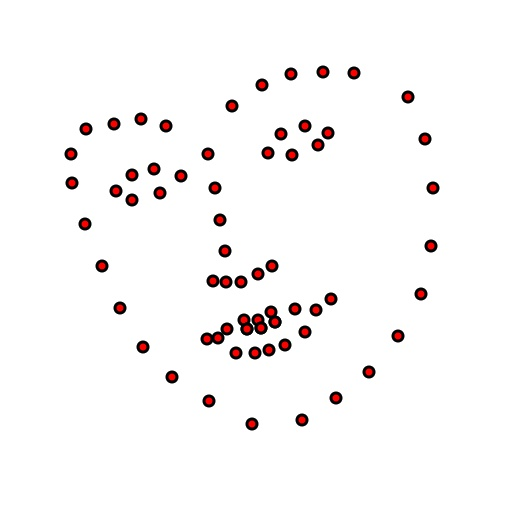
\includegraphics[width=\textwidth]{resources/landmark}
        \caption{Spare landmarks}
    \end{subfigure}
    ~~~~~~~~~
    \begin{subfigure}[b]{0.15\textwidth}
            
\includegraphics[width=\textwidth]{resources/svs}
        \caption{Visualise decision function trained}
        \label{fig:svs}
    \end{subfigure}
    \caption{Decision function trained on sparse landmarks}
    \label{fig:build_svs}
\end{figure}





% ---------------------------------------------------------------------------------------------------------------------------------------------------


\subsection{Shape Flow}

With decision functions built from training data, the second module designed to register all decision functions to mean shape, we named it Shape Flow. Shape Flow is introduced based on optical flow, which generate pixel-wise correspondences for video sequences. Optical flow works for video sequences based on assumptions e.g. brightness constancy and motion smoothness. However, in terms of shapes, neither constant illumination nor continuous motion exists in sequence of shapes as all training data are independent. Thus we proposed shape flow with subspace constrains introduced from trajectories.

\subsubsection{Trajectory Basis} \label{sec:trabasis}
Since shapes from training data set having completely no motion smoothness, it is of importance to contain constrains in optimization on how pixels moves from one shape frame to another. We constrain the optimization on trajectory subspace.
We supervise trajectories from sparse landmarks. To begin with, Non-rigid Iterative Closest Point (NICP)\cite{?} applied on sparse annotated points. NICP deforms target points to fit the template iteratively until all points on target deformed to match points on template. Performs the algorithm for all training data will get an implicit point correlation between sparse shapes.

Since optical flow pixel-wise frame registration, the trajectory basis build should also matches the dimension, which is dense on shapes with trajectory length depends on number of training data. With correspondences produced after applying NICP, Thin-Plate Spline (TPS)\cite{?} transformations are utilized to warp every shape planes to template plane thereby generates an implicit dense shape registering. For all dense transformations $\bm{u_n}(\bm{x}), n \in {1,...,F}$, where $F$ is number of data and $\bm{x}$ is vector of pixels, Principle Component Analysis (PCA) is performed on trajectory to obtain low rank trajectory basis:
\begin{equation}
    \begin{bmatrix}
        \bm{u_1}(\bm{x}) \\
        \vdots \\
        \bm{u_F}(\bm{x})
    \end{bmatrix}
    =
    \begin{bmatrix}
        \bm{q_1}(1) & \cdots & \bm{q_R}(1) \\
        \vdots      & \ddots & \vdots  \\
        \bm{q_1}(F) & \cdots & \bm{q_R}(F)
    \end{bmatrix}
    \times
    \begin{bmatrix}
        \bm{v_1}(x) \\
        \vdots \\
        \bm{v_R}(x)
    \end{bmatrix}
\end{equation}
where $\bm{q_i}(n)$ are low rank components with $R \ll 2F$ and $\bm{v_i}(x)$ weighted each component with dependencies on $x$. Simpler expression shown below:
\begin{equation}
    \bm{u_n}(\bm{x})=\sum_{i=1}^R\bm{q_i}(n)\bm{v_i}(x)+\bm{\varepsilon_n}(\bm{x})
\end{equation}
Although optical flow on shapes made under the assumption that objects motion are smooth, the low rank constrain on trajectory basis recovered the hypothesis.

\subsubsection{Algorithm}
To register all decision functions to template shape, decision function $d_i(\bm{x}), i \in {1,...,F}$ are grouped into one sequence before applying flow algorithm. The objective cost function we would like to minimise is:
\begin{align}
    E[\bm{u_n}(\bm{x}), \bm{v}]&=\alpha \int_{\Omega}\sum_{n=1}^F|\bm{d_n}(x+\bm{u_n}(x))-\bm{d_0}(x)\| dx  \label{eq:costfunc}\\
    &+ \beta \int_{\Omega}\sum_{n=1}^F\|\bm{u_n}(x)-\sum_{i=1}^R\bm{q_i}(n)\bm{v_i}(x)\|^2 dx \label{eq:lowrank}\\
    &+ \sum[\bm{TV}(Qv)]  + v^T.L.v
\end{align}
where $d_n(x)$ is the decision function from~\eqref{eq:decisionfunc}, which returns possibilities of given coordinate classified as shape compunent. $TV(Qv)$ is total variation as regularization on low rank subspace, $Q$ is trajectory basis and $v^T.L.v$ is low rank spacial constrains.

Term~\eqref{eq:costfunc} state the shape constancy where points having similar classification probability are from same object.
Part~\eqref{eq:lowrank} applies constrain on low rank trajectory basis states in section~\ref{sec:trabasis}.
The objective cost function has two free parameters $u$ and $v$, so we performs alternating minimisation. The equation can be solved using thresholding scheme as used in \cite{?} after linearisation of image functions. The minimisation can be speed up by paralleling the minimisation for every spatial-temporal point $(x;n), x \in \Omega, n \in {1,...F}$ independently.

After solving the equation, $\bm{u_n}(\bm{x}), x \in \Omega$ gives a group of dense deformations that registering every decision functions in the shape sequence to reference frame e.g. $\bm{u_1}(\bm{x})$ registers decision function $\bm{d_1}(\bm{x})$ to the reference frame. Applying PCA on deformations gives dense deformable shape model.


\subsubsection{Computational Complexity?}


\clearpage